\section{State Rankings}

Using the statistical and (in)distinguishability graph methods described in \cref{sec:stats_methods}, we were able to develop both graph visualizations of state distinguishability and a possible ranking of the states.

\begin{figure}[h]
    \centering
    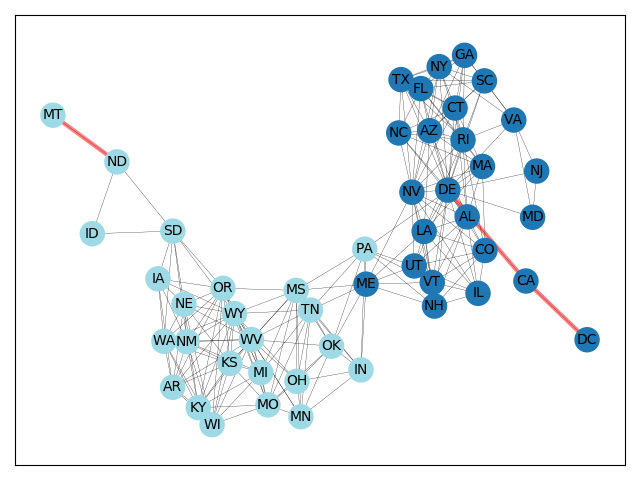
\includegraphics{caida/caida_network_invalid_comps.png}
    \caption{Indistinguishability graph of traceroute data as aggregated by state}
    \label{fig:caida_network_invalid_comps}
\end{figure}

\Cref{fig:caida_network_invalid_comps} shows an indistinguishability graph of comparisons between the states (previously seen in \cref{sec:stats_methods}), where node colors correspond to communities and bold red lines correspond to bridges.\footnote{Bridges can be thought of as indicators of comparison quality; any state on the end of a bridge can be compared to all but one of the other states.} As noted earlier, this graph has no disjoint subgraphs, so ranking by clusters is not possible. \Cref{fig:caida_network_valid_comps} shows the corresponding distinguishability graph, which is much more connected, indicating this data is a good candidate for the topological sort method.

\begin{figure}[h]
    \centering
    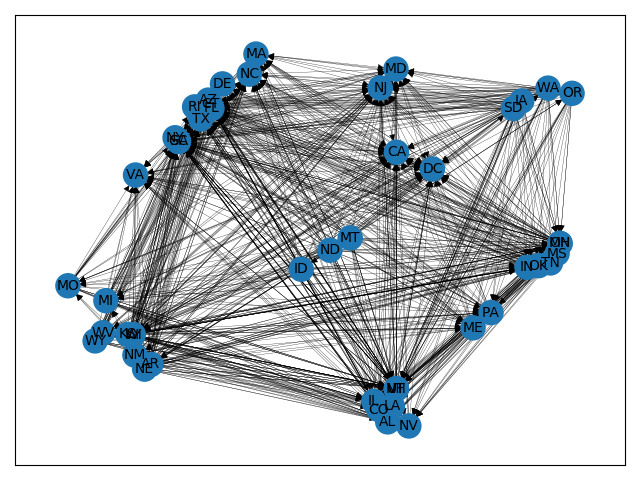
\includegraphics{caida/caida_network_valid_comps.png}
    \caption{Distinguishability graph of traceroute data as aggregated by state}
    \label{fig:caida_network_valid_comps}
\end{figure}

When sorted we obtain a list of 49 states (including the District of Columbia; Hawaii and Alaska were unreachable); two states were not reachable by a maximal topological sort (described in \cref{sec:methods_stats_topological_rankings}). \Cref{tab:caida_topological_state_rankings} shows this ranking, which roughly confirms what we would expect based on prior notions and the heatmaps. Since the topological sort method is based on a graph interpretation and not a traditional sort of means or medians, those values are not shown alongside the states.

\begin{table}[h]
    \centering
    \begin{longtable}{ll|ll|ll|ll|ll}
        \textbf{Rank} & \textbf{State} & \textbf{Rank} & \textbf{State} & \textbf{Rank} & \textbf{State} & \textbf{Rank} & \textbf{State} & \textbf{Rank} & \textbf{State} \\
        \midrule
        \endhead
        \midrule
        \multicolumn{10}{r}{{Continued on next page}} \\
        \endfoot
        \endlastfoot
        \textbf{1 } & DC & \textbf{11} & TX & \textbf{21} &  LA & \textbf{31} & TN & \textbf{41} &    WY \\
        \textbf{2 } & DE & \textbf{12} & AL & \textbf{22} &  NV & \textbf{32} & MN & \textbf{42} &    NE \\
        \textbf{3 } & MD & \textbf{13} & CT & \textbf{23} &  PA & \textbf{33} & OH & \textbf{43} &    NM \\
        \textbf{4 } & CA & \textbf{14} & RI & \textbf{24} &  VT & \textbf{34} & WI & \textbf{44} &    OR \\
        \textbf{5 } & NJ & \textbf{15} & NC & \textbf{25} &  NH & \textbf{35} & KY & \textbf{45} &    IA \\
        \textbf{6 } & NY & \textbf{16} & MA & \textbf{26} &  UT & \textbf{36} & KS & \textbf{46} &    WA \\
        \textbf{7 } & SC & \textbf{17} & AZ & \textbf{27} &  IN & \textbf{37} & MO & \textbf{47} &    ID \\
        \textbf{8 } & GA & \textbf{18} & IL & \textbf{28} &  WV & \textbf{38} & MI & \textbf{48} &    MT \\
        \textbf{9 } & VA & \textbf{19} & CO & \textbf{29} &  MS & \textbf{39} & AR & \textbf{49} &    ND \\
        \textbf{10} & FL & \textbf{20} & ME & \textbf{30} &  OK & \textbf{40} & SD &             &       \\
        \caption{CAIDA+Atlas topologically sorted state rankings}
        \label{tab:caida_topological_state_rankings}
    \end{longtable}
\end{table}

\begin{figure}[h]
    \centering
    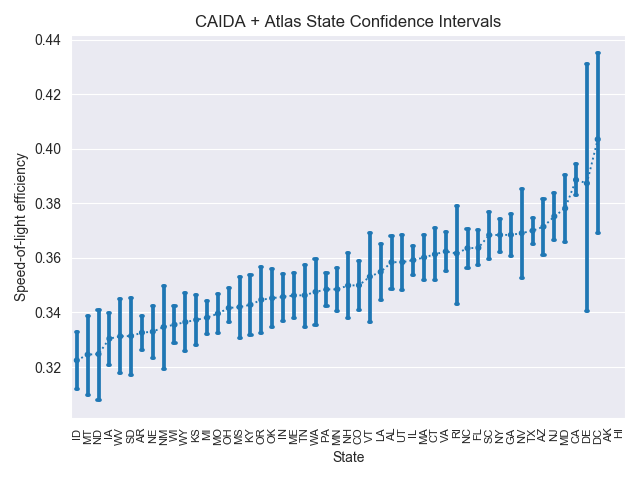
\includegraphics{images/comparative/confidence_intervals/caida_confidence_interval.png}
    \caption{Traceroute confidence intervals for rankings; higher is better}
    \label{fig:caida_confidence_intervals}
\end{figure}

\Cref{fig:caida_confidence_intervals} shows an alternate way of displaying state ranks, using the mean of each state for comparisons. Since data for each state does not follow a normal distribution (see \cref{sec:comparative-distribution} for a variety of \kdes on the subject) the bootstrapping method was used to calculate confidence intervals. Loosely speaking, for each state the "true" mean could be anywhere between the upper and lower bounds of the intervals.
